%!TEX root = ../../main.tex

\chapter{\Pl Setup}	\label{ch::pl_setup}
\chaptermark{PL Setup}

	The key measurements of this thesis are spectroscopic measurements of \sivs in nanodiamonds.
	For this aim, a home-built confocal setup is used, which is described in this chapter.

	The confocal setup serves to perform a series of spectroscopic measurements on \fl: scanning the sample to find \sivs, recording \pl spectra of the aforementioned, determining the brightness of an emitter by recording the saturation count rate \todo[fancyline]{saturation already introduced?}, and determine whether the emitter in question is a single emitter by performing photon autocorrelation (\gt) measurements.
	The entire setup is built up by a confocal setup, to which a spectrometer or an \HBT setup are attached: 

	\begin{itemize}
		\item The confocal setup is the core component where the sample sits. 
		The  excitation laser light is focused on the sample by an objective and the \fl from the \sivs collected by the same objective, hence the name confocal.
		The sample can ge moved to scan ist in order to excite emitters and collect the \fl.
		For scanning, and \apd is attached to the confocal setup.
		\item The grating spectrometer to investigate the spectral properties of the emitters. This is crucial to distinguish between \sivs, other \ccs and \nds which do not host color centers.
		\item A \keyword{\HBT} (\hbt) setup to investigate the single photon character. It is built up of two \apds (\APDs) which are also used for scanning the sample and for performing saturation measurements.
	\end{itemize}

	\begin{figure}[t] %fig::confocal_setup
		\begin{minipage}{.5\textwidth}
			\centering
			\testbox{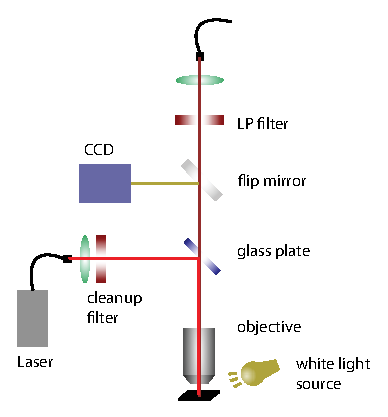
\includegraphics{./pics/confocal_setup_small.eps}}
			\caption{Confocal setup}
			\label{fig::confocal_setup}
		\end{minipage}
		\hfill
		\begin{minipage}{.5\textwidth}
			\centering
			\testbox{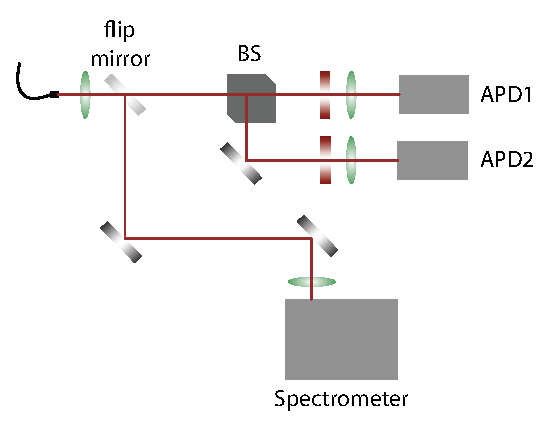
\includegraphics{./pics/hbt_spectrometer.eps}}
			\caption{HBT, spectrometer}
			\label{fig::hbt_spectrometer}
		\end{minipage}
	\end{figure}	


	\section[Confocal Setup]{Confocal Setup} \label{sec::confocal}

		\autoref{fig::confocal_setup} depicts a sketch of the confocal setup. 
		Except for the laser and the sample stage, the whole setup is fixed to a vertical breadboard. 
		As this vertical design permits a horizontal sample stage, it allows for easy scanning and exchanging of the samples, without the need of gluing them to a vertical stage.
		The friction between the sample and the aluminum surface of the stage is sufficient that the sample does not get out of place during scanning.
		For some measurements it is important that the sample has a a defined orientation.
		For this purpose it is possible to orient it with the help of an aluminum angle an adjust the orientation with a manual rotation stage. 
		In contrast, the translation stage is powered with two stepper motors Newport MVP25XL) in the horizontal x and y directions.
		Above the horizontal stage, the objective is fixed to another stage which in turn is fixed to the vertical breadboard.
		In this way, the vertical z distance can be adjusted for focusing the laser light on the sample.
		It also enables scanning in the direction of the optical axis, which is coincides with the height of the sample.
		Therefore, three-axis scanning of the sample is implemented.

		The bright red color in the sketch in \autoref{fig::confocal_setup} represents the excitation beam path.
		The sample is excited with a continuous wave diode laser (Sch\"after-Kirchhoff, 58FCM) which emits at a \wl of \SI{660}{\nano\meter}.
		The outlet of the laser is a pigtail fiber.
		The laser light is outcoupled and collimated exploiting an aspheric lens.
		To suppress sideband emission from the laser, a \SI{660}{\nm} bandpass filter with a filter window of  \SI{10}{\nm} is used.
		After this cleanup filter, the excitation beam then hits a glass plate (fabricator Halle Germany \todo[fancyline]{thickness}) which guides the beam through a microscope objective to be focused on the sample.
		The microscope objective is of the type Olympus, LMPlanFLN 100x and has a numerical aperture of 0.8.
		As the luminescence light from the emitter is in the same focus as the excitation laser light, it is effectively collected by the objective (hence "confocal setup").

		The collected light follows the detection beam path depicted in dark red in \autoref{fig::confocal_setup}.
		Both the excitation light reflected from the sample surface and the \fl from the color centers pass through the glass plate.
		If the flip mirror behind the beamsplitter is taken out of the beam path, the beamis directed towards a single mode fiber which connects the confocal setup with either the spectrometer or the \hbt setup. 
		In front of the \smf there is a longpass filter to filter out the residual excitation light and also ambient light.
		The filter is chosen with a cutoff \wl of \SI{710}{\nm} or \SI{720}{\nm}.
		The \fl is fed into the single-mode fiber (Thorlabs SM600) with an aspheric lens.
		Besides the obvious purpose of guiding the \pl light to the spectrometer and the \HBT setup for spectroscopic investigations, it has another crucial application:
		Its diameter of about \SI{4.3}{\micro\meter} serves as a pinhole to reject \pl light from depths ouside of the focal plane \cite{Santori2010}. 
		For this axis the resolution amounts to \todo[fancyline]{value}, in the plane of the sample it is \todo[fancyline]{value}.
		\todo[fancyline]{short discussion if resolution is enough}

		According to the experimental necessities, instead of the mentioned glass plate a dichroic mirror (DRLP692) can be employed.
		The dichroic mirror spectrally separates excitation light from \pl light as it selectively transmits and reflects sight as a function of its wavelength. 
		The glass plate features a high transmission of 90\%\todo[fancyline]{check number} and therefore exhibits a high collection efficiency of \fl, but at the same time, 90\% of the excitation light is lost, as it is not reflected towards the sample.
		In contrast to that the dichroic mirror allows for a higher excitation intensity using the same excitation laser which is necessary for instance for saturation measurements. 
		However, a high excitation intensity may cause permanent fluorescence intermittence of the \sivs (for further detail, refer to \todo[fancyline]{insert chapter}).
		In general, if a high excitation is necessary, as for saturation measurements, the dichroic mirror is used; otherwise, the glass plate is used to collect as much \fl as possible without damaging the \sivs due to exposure to a high laser light intensity.

	\section[Optical Imaging]{Optical Imaging of The Sample Surface} \label{sec::methods_optical}

		The confocal can be modified to investigate the sample surface before starting the fluorescence measurements.
		For this purpose, the sample is directly illuminated in a flat angle from outside the objective with white light from a halogen lamp (depicted as white light source in \autoref{fig::confocal_setup}). 
		The flip mirror behind the glass plate is brought into an upright position to guide the light towards a CCD camera (\todo[fancyline]{specs}).
		The scattered light from the sample surface is collected by the objective and the surface is imaged on the CCD chip \todo[fancyline]{resolution CCD}.
		Hence \Nds and other features on the substrate are visible.
		The resolution of this configuration of the setup is limited by \todo[fancyline]{optical diffraction, shadows}.
		\\
		In chapter \autoref{} an application of the \nd is introduced, for which it is of major importance to know the position of specific \nds.
		Therefore, cross markers are milled into the surface of the substrate on which the \nds are situated.
		These markers of a size of \SI{10}{\micro\meter} can easily be recognized by optical iamging.
		The starting point for a scan of an area of interest on the sample is fixed while navigating with the optical image.
		After flipping the flip mirror, a \pl scan of that area is started.

	\section[Spectrometer]{Spectrometer} \label{sec::methods_spectrometer}

		\autoref{fig::hbt_spectrometer} displays the detection part of the setup.
		The \fl from the fiber which connects the confocal setup with the detection setup is outcoupled with an aspheric lens. 
		A flip mirror is employed to direct the light either to a grating spectrometer or the \hbt setup.
		The optical spectrum of a light source gives insight to the optically active constituents and therefore bears information about the emitter.
		\\
		As mentioned before, the \fl from the \sivs is investigated with the grating spectrometer (Princeton Instruments Acton2500i).
		The incident beam passes through an entrance slit, is then scattered on the grating where the light is spectrally divided and finally hits a detector, imaging the entrance slit on the detector surface.
		The employed detector is a CCD camera ()\todo[fancyline]{type} which is cooled with liquid nitrogen to a temperature of \SI{-120}{\celsius} for background reduction due to thermally generated free charge carriers.
		It is optimized for detection of light up to a \wl of \SI{900}{nm}.
		The spectrometer features three gratings: \SI[per-mode=symbol]{600}{\lines\per\mm}, \SI[per-mode=symbol]{1200}{\lines\per\mm}, and \SI[per-mode=symbol]{1800}{\lines\per\mm}.
		These gratings are mounted on a turret, allowing easy switching of the gratings between measurements.
		\\
		With the spectrometer's step-and-glue function which is implemented in the spectrometer software (WinSpec) it is possible, to record several spectra over a wide \wl range which are then stiched together.
		It is therefore possible to combine a larger \wl range with a higher resolution.
		For most measurements the grating with \SI[per-mode=symbol]{600}{\lines\per\mm} was used. 
		The resolution of the spectrometer using the \SI{600}{\lines\per\mm} is \SI{0.13}{nm} at \SI{738}{nm} and the accuracy amounts to \num{\pm0.4} as stated by the manufacturer.
		This resolution suffices for most of the measurements mentioned in this work.

	\section[HBT]{\HBT Setup}\label{sec::methods_hbt}

		A \majorkeyword{\HBT setup} serves to record the \keyword{photon autocorrelation function} (\keyword{\gt function}) of an emitter.
		In this work, the \gtf is used to make statements about whether a \pl source emits single photons and is therefore one single emitter.
		In the photon number representation, it is defined as follows:
		\[
		\gtz = \frac{ \mean{ N(t) N(t+\tau) } }{\mean{N(t)}^2}.
		\]
		Here, $N(t)$ denotes the photon at a certain time $t$, $N(t+\tau)$ denotes the photon at a time interval $\tau$ later than $t$.
		The angular brackets $\mean{}$ denote the temporal averaging.
		The physical explanation is \todo[fancyline]{fox nachlesen} that if the source is a single emitter and emits a photon at a  time $t$, the next time any photon is recorded is at time $t+\tau$.
		For a time interval close to zero, the value of the \gtf must ideally approach zero or at least be smaller than \num{0.5} if only a single emitter is present:
		The denominator is zero, because $N(t + \tau) (\tau = 0)=0$ due to only one photon, namely $N(t)$ being present.
		If two photons are emitted at the same time (time delay zero), the \gtf yields $\gtz=0.5$. 
		(For a detailed explanation of the \gtf read \cite{Fox2006})
		\\
		The principle of the \hbt setup is to evaluate the time delay between two consecutive photons. 
		A sketch of the \hbt setup is shown in \autoref{fig::hbt_spectrometer}.
		The photons are detected with single photon \apds (\APDs) of the type PicoQuant $\tau${}-SPAD100.
		\APDs are the semiconductor analog to photomultiplier tubes:
		An incoming photon creates secondary charge carriers through ionization.
		The secondary charge carrier is accelerated by a bias voltage to create more secondary charge carriers, resulting in an avalanche effect.
		Therefore, the signal of a single photon is intensified and detected as an electrical current pulse.
		These \apds have a nominal detection efficiency of up to 70\% at an optimal wavelength of about \SI{670}{\nm} and a dark count rate of under \SI{100}{\cps}.
		If a charge carrier created by the avalanche is trapped and later liberated, it induces a so-called afterpulse.
		To avoid detecting these artifacts as real events, the \APDs have a dead time of about \SI{70}{\ns}.
		In the ideal case, one \APD would be enough to measure the time delay between two consecutive photons. 
		However, the second of two consecutive photons could hit the detector during its dead time.
		To circumvent this problem, two \APDs are employed and the detection beam is split with a non-polarizing 50:50 beamsplitter cube.
		Each beam then passes through a bandpass filter and is focused on the \apd with an aspheric lens.
		As the beam path is slightly different for each \APD, a small optical path difference is introduced, however, this difference only results in an offset of the \gtf and does not alter the physical nature of the result.
		The bandpass filters serve two purposes:
		First, they limit optical crosstalk between the \apds. 
		The detection process in an \apd produces light due to recombination of charge carriers. 
		Crosstalk between two \apds occurs, if one of the photons produced by recombination in one \apd escapes and is detected in the other one \cite{Younger2009}.  
		Secondly, the bandpass filters serve to reduce \bkg during the \gt measurement process or to spectrally divide emission from several emitters.
		Therefore, it is possible to find single emitters, which are not spatially separated enough to be separated by the spatial resolution of the setup:
		They can be individually investigated if their \ZPLs exhibit wavelengths which are spectrally well seperated.
		Bandpass filters suited for the respective wavelengths are used to investigate light from one of the \ZPLs.
		\\
		When the \APD fires, it outputs a digital TTL (transistor-transistor logic compatible) signal. 
		The arrival times of the signals (so-called time tags) are recorded with a time tag unit (produced by dotfast-consulting, timing resolution \SI{78.125}{\pico\second}).
		The timing uncertainty of the photon detection process introduces variations of the digital signal's time tag from the actual detection time.
		Note that this error does not represent the time evolving from the photon impact to recording, but solely the uncertainty of the exact recording time.
		This process is called timing jitter.
		It affects the time tags and with them the physical nature\todo[fancyline]{wording} of the \gtf.
		A discussion of the impact of timing jitter will be given in \autoref{ch::g2}. \todo[fancyline]{put in reference}
		\\
		As stated earlier, the time delay between two consecutive photons is necessary for the reconstruction of the \gtf.
		The time delays are fed into a histogram which is then fitted to receive the continuous \gtf.
		In the \HBT{}-setup the arrival time of the photons are measured with two |APDs and for each \APD one list of arrival times is recorded as raw data.
		To get a single array of arrival times of the photons, which can then be binned to obtain the \gtf, the arrays of time tags of the two \APDs have to be correlated.
		For that, the time difference between each entry in one array and all consecutive time tags in the other array are determined and stored according a binning defined by the the timing resolution of the time tag unit.
		After normalizing and fitting these data, statements about whether the emitter is a single emitter can be made.





